
\textcolor{red}{hay que mejorar los graficos y sacar de todos lados los TIKZ, que se compilen afuera del codigo del texto}


\begin{definition}  
\textbf{Conjunto elemental en } $\mathbb{R}^3$.  Un conjunto acotado $W\subseteq\mathbb{R}^3$ se llama \emph{elemental} si puede ser descrito de alguna de las siguientes maneras:

\begin{enumerate}
    \item Existen $D_1 \subset  \mathbb{R}^2 $ un conjunto elemental y funciones  $\eta_{11},\; \eta_{21}: D_1\to\R$  continuas  tales que $$\eta_{11}(x, y) <  \eta_{21}(x, y)  \: \forall (x,y) \in  (D_1)^{\circ}$$ y \begin{equation}\label{def_conj_elem_R3_t1} W = \left\{ (x, y, z) \in \mathbb{R}^3 \;\middle|\;  (x,y) \in D_1 \: \land  \: \eta_{11}(x, y) \leq z \leq \eta_{21}(x, y)  \: \forall (x,y) \in D_1 \right\}.\end{equation}
\begin{figure}[htbp]
    \centering
    % Llamamos al archivo con el código TikZ extraído
    
    \centering
% \tikzsetnextfilename{conj_elemental1_R3}
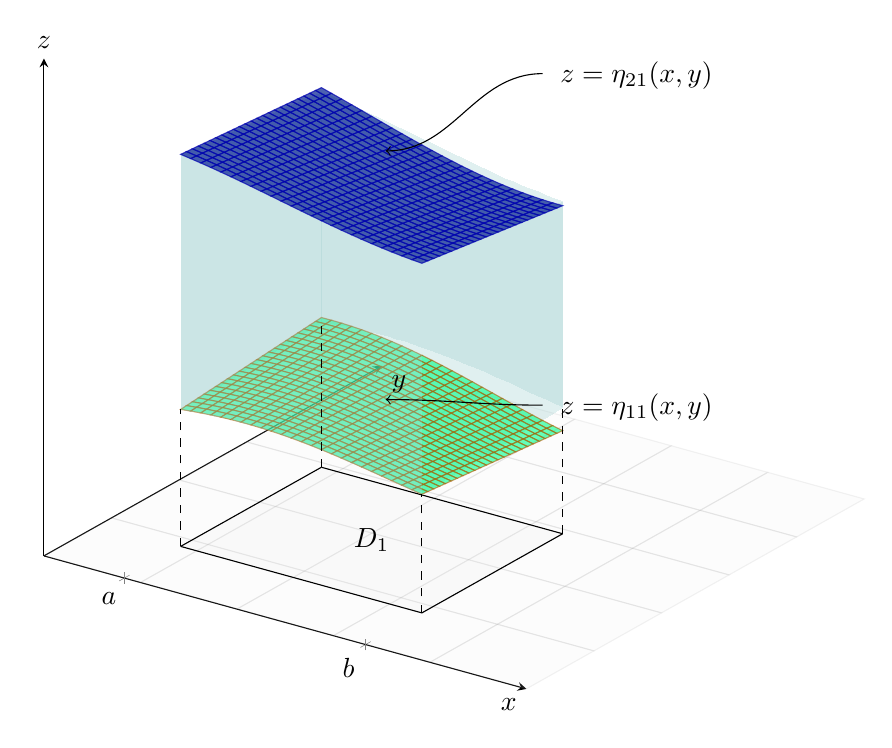
\begin{tikzpicture}
    \begin{axis}[
        view={35}{25}, % Ángulo de perspectiva
        width=12cm, height=12cm,
        grid=none,
        axis lines=center,
        xmin=0, xmax=6,
        ymin=0, ymax=6,
        zmin=0, zmax=6,
        xtick={1,4}, xticklabels={$a$,$b$}, % Marcas exactas de a y b en el eje x
        ytick=\empty, ztick=\empty,
        xlabel={$x$}, ylabel={$y$}, zlabel={$z$},
        every axis x label/.style={at={(ticklabel* cs:1)},anchor=north east},
        every axis y label/.style={at={(ticklabel* cs:1)},anchor=north west},
        every axis z label/.style={at={(ticklabel* cs:1)},anchor=south},
        clip=false
    ]

    % --- 0. Grilla en el piso (z=0) ---
    \addplot3 [surf, domain=0:6, domain y=0:6, samples=6, samples y=6, opacity=0.1, point meta=0, colormap={fondogris}{color=(gray!25) color=(gray!25)}, shader=faceted, faceted color=gray] (x,y,0);

    % --- 1. Dominio D_1 en R2 (Plano z=0) ---
    \addplot3 [surf, domain=1:4, domain y=0:1, samples=30, opacity=0.15, colormap={gray}{color=(gray!15) color=(gray!15)}, shader=interp, draw=none] 
        (x, {1 + 2.5*y}, 0);

    % Contorno de D1 (borde recto, uniendo las esquinas de la sombra)
    \draw[thin, black] (1, 1, 0) -- (4, 1, 0);
    \draw[thin, black] (1, 3.5, 0) -- (4, 3.5, 0);
    \draw[thin, black] (1, 1, 0) -- (1, 3.5, 0);
    \draw[thin, black] (4, 1, 0) -- (4, 3.5, 0);

    % --- 2. Paredes laterales (Efecto sólido) ---
    % Pared trasera
    \addplot3 [surf, domain=1:4, domain y=0:1, samples=30, opacity=0.3, colormap={teal}{color=(teal!40) color=(teal!40)}, shader=interp, draw=black!70] 
        (x, 3.5, { (1-y)*(1.5 + 0.2*sin(x*50) + 0.1) + y*(4.5 + 0.3*cos(x*40) - 0.2) });

    % Pared izquierda (en x=a)
    \addplot3 [surf, domain=0:1, domain y=0:1, samples=5, opacity=0.3, colormap={teal}{color=(teal!40) color=(teal!40)}, shader=interp, draw=black!70] 
        (1, {1 + 2.5*x}, { (1-y)*(1.5 + 0.2*sin(50) + 0.1*x) + y*(4.5 + 0.3*cos(40) - 0.2*x) });

    % Pared derecha (en x=b)
    \addplot3 [surf, domain=0:1, domain y=0:1, samples=5, opacity=0.3, colormap={teal}{color=(teal!40) color=(teal!40)}, shader=interp, draw=black!70] 
        (4, {1 + 2.5*x}, { (1-y)*(1.5 + 0.2*sin(200) + 0.1*x) + y*(4.5 + 0.3*cos(160) - 0.2*x) });

    % --- 3. Tapas del sólido ---
    % ¡AHORA SÍ!: Tapa inferior forzada a NARANJA plano con un mapa de color puro
    \addplot3 [surf, domain=1:4, domain y=0:1, samples=25, opacity=0.6, 
               colormap={pureorange}{rgb255=(0,255,140,0) rgb255=(1,255,140,0)}, shader=flat, draw=orange!70!black] 
        (x, {1 + 2.5*y}, { 1.5 + 0.2*sin(x*50) + 0.2*y*cos(x*40) });
        
    % Pared frontal
    \addplot3 [surf, domain=1:4, domain y=0:1, samples=30, opacity=0.3, colormap={teal}{color=(teal!40) color=(teal!40)}, shader=interp, draw=black!70] 
        (x, 1, { (1-y)*(1.5 + 0.2*sin(x*50)) + y*(4.5 + 0.3*cos(x*40)) });

    % Tapa superior forzada a AZUL plano con su propio mapa puro
    \addplot3 [surf, domain=1:4, domain y=0:1, samples=25, opacity=0.7, 
               colormap={pureblue}{rgb255=(0,30,144,255) rgb255=(1,30,144,255)}, shader=flat, draw=blue!70!black] 
        (x, {1 + 2.5*y}, { 4.5 + 0.3*cos(x*40) - 0.3*y*sin(x*30) });

    % --- 4. Esquinas y proyecciones (Líneas punteadas de soporte) ---
    \draw[dashed, thin] (1, 1, 0) -- (1, 1, {1.5 + 0.2*sin(50)});
    \draw[dashed, thin] (4, 1, 0) -- (4, 1, {1.5 + 0.2*sin(200)});
    \draw[dashed, thin] (1, 3.5, 0) -- (1, 3.5, {1.5 + 0.2*sin(50) + 0.1});
    \draw[dashed, thin] (4, 3.5, 0) -- (4, 3.5, {1.5 + 0.2*sin(200) + 0.1});

    % --- 5. Etiquetas ---
    \node at (2.5, 2.25, 0) {$D_1$};

    % Etiquetas de las superficies
    \node[anchor=west] at (3.5, 4, 5.2) {$z = \eta_{21}(x,y)$};
    \node[anchor=west] at (3.5, 4, 1.2) {$z = \eta_{11}(x,y)$};
    
    % Flechas a las superficies
    \draw[->, out=180, in=0, thin] (3.4, 4, 5.2) to (2.5, 2.5, 4.6);
    \draw[->, out=180, in=0, thin] (3.4, 4, 1.2) to (2.5, 2.5, 1.6);

\end{axis}
\end{tikzpicture}
\caption{Conjunto elemental de Tipo I.}
 
    \label{fig:conjunto tipo 1}
\end{figure}
\end{enumerate}
\end{definition}


\begin{itemize}
    \item Existen $D_2 \subset \mathbb{R}^2$ un conjunto elemental y funciones $\eta_{12},\; \eta_{22}: D_2\to\mathbb{R}$ continuas tales que 
    \[
    \eta_{12}(x, z) < \eta_{22}(x, z) \quad \forall (x,z) \in (D_2)^{\circ}
    \]
    y 
    \begin{equation}
        \label{def_conj_elem_R3_t2} 
        W = \left\{ (x, y, z) \in \mathbb{R}^3 \;\middle|\; (x,z) \in D_2 \: \land \: \eta_{12}(x, z) \leq y \leq \eta_{22}(x, z) \: \forall (x,z) \in D_2 \right\}
    \end{equation}
\end{itemize}

\begin{figure}[htbp]
    \centering
    % Llamamos al archivo con el código TikZ extraído
    \tikzexternaldisable
    \centering
    \tikzsetnextfilename{conj_elemental2_R3}
    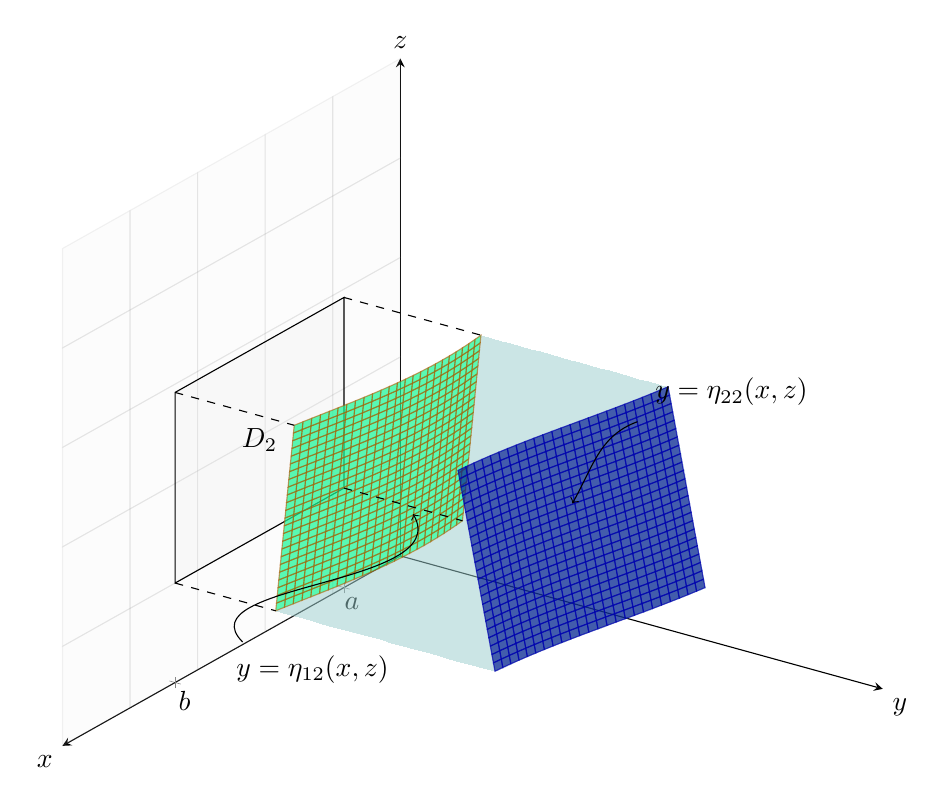
\begin{tikzpicture}
    \begin{axis}[
        view={125}{25}, % Rotado para que el sólido "venga" hacia adelante
        width=12cm, height=12cm,
        grid=none,
        axis lines=center,
        xmin=0, xmax=6,
        ymin=0, ymax=6, % Eje de profundidad y proyectado
        zmin=0, zmax=6,
        xtick={1,4}, xticklabels={$a$,$b$},
        ytick=\empty, ztick=\empty,
        xlabel={$x$}, ylabel={$y$}, zlabel={$z$},
        every axis x label/.style={at={(ticklabel* cs:1)},anchor=north east},
        every axis y label/.style={at={(ticklabel* cs:1)},anchor=north west},
        every axis z label/.style={at={(ticklabel* cs:1)},anchor=south},
        clip=false
    ]

    % --- 0. Grilla de fondo (plano xz en y=0) ---
    \addplot3 [surf, domain=0:6, domain y=0:6, samples=6, samples y=6, opacity=0.1, point meta=0, colormap={fondogris}{color=(gray!25) color=(gray!25)}, shader=faceted, faceted color=gray] (x,0,y);

    % --- 1. Dominio D_2 en R2 (Plano xz) ---
    % Relleno de D2
    \addplot3 [surf, domain=1:4, domain y=1.2:3.5, samples=2, opacity=0.15, colormap={gray}{color=(gray!20) color=(gray!20)}, shader=interp, draw=none] 
        (x, 0, y);
    % Contorno de D2 (borde recto)
    \draw[thin, black] (1, 0, 1.2) -- (4, 0, 1.2) -- (4, 0, 3.5) -- (1, 0, 3.5) -- cycle;

    % --- 2. Paredes del volumen (Relleno completo de las 4 caras laterales) ---
    % Pared en z = 3.5 (Toma en cuenta z=3.5 para cerrar perfecto con el techo)
    \addplot3 [surf, domain=1:4, domain y=0:1, samples=20, opacity=0.3, colormap={teal}{color=(teal!40) color=(teal!40)}, shader=interp, draw=black!70]
        (x, { (1-y)*(1.2 + 0.2*sin(x*50) + 0.1*3.5) + y*(4.5 + 0.3*cos(x*40) - 0.2*3.5) }, 3.5);
    % Pared en z = 1.2 (Toma en cuenta z=1.2 para cerrar perfecto con el techo)
    \addplot3 [surf, domain=1:4, domain y=0:1, samples=20, opacity=0.3, colormap={teal}{color=(teal!40) color=(teal!40)}, shader=interp, draw=black!70]
        (x, { (1-y)*(1.2 + 0.2*sin(x*50) + 0.1*1.2) + y*(4.5 + 0.3*cos(x*40) - 0.2*1.2) }, 1.2);
    % Pared en x = a (x=1)
    \addplot3 [surf, domain=1.2:3.5, domain y=0:1, samples=20, opacity=0.3, colormap={teal}{color=(teal!40) color=(teal!40)}, shader=interp, draw=black!70]
        (1, { (1-y)*(1.2 + 0.2*sin(50) + 0.1*x) + y*(4.5 + 0.3*cos(40) - 0.2*x) }, x);
    % Pared en x = b (x=4)
    \addplot3 [surf, domain=1.2:3.5, domain y=0:1, samples=20, opacity=0.3, colormap={teal}{color=(teal!40) color=(teal!40)}, shader=interp, draw=black!70]
        (4, { (1-y)*(1.2 + 0.2*sin(200) + 0.1*x) + y*(4.5 + 0.3*cos(160) - 0.2*x) }, x);

    % --- 3. Superficie Trasera y = eta12 ---
    \addplot3 [surf, domain=1:4, domain y=1.2:3.5, samples=25, opacity=0.6,
               colormap={pureorange}{rgb255=(0,255,140,0) rgb255=(1,255,140,0)}, shader=flat, draw=orange!70!black]
        (x, { 1.2 + 0.2*sin(x*50) + 0.1*y }, y);

    % --- 4. Superficie Delantera y = eta22 (Mirando al frente) ---
    \addplot3 [surf, domain=1:4, domain y=1.2:3.5, samples=25, opacity=0.7,
               colormap={pureblue}{rgb255=(0,30,144,255) rgb255=(1,30,144,255)}, shader=flat, draw=blue!70!black]
        (x, { 4.5 + 0.3*cos(x*40) - 0.2*y }, y);

    % --- 5. Proyecciones punteadas al plano (una por cada esquina de D2) ---
    \draw[dashed, thin] (1,0,1.2) -- (1, {1.2 + 0.2*sin(50) + 0.1*1.2}, 1.2);
    \draw[dashed, thin] (4,0,1.2) -- (4, {1.2 + 0.2*sin(200) + 0.1*1.2}, 1.2);
    \draw[dashed, thin] (1,0,3.5) -- (1, {1.2 + 0.2*sin(50) + 0.1*3.5}, 3.5);
    \draw[dashed, thin] (4,0,3.5) -- (4, {1.2 + 0.2*sin(200) + 0.1*3.5}, 3.5);

    % --- 6. Etiquetas y flechas (ajustadas para que no tapen la figura) ---
    \node at (2.5, 0, 2.35) {$D_2$};
    
    % Flecha para la cara delantera (techo)
    \node[anchor=south west] at (3.5, 5.5, 4.5) {$y = \eta_{22}(x,z)$};
    \draw[->, thin] (3.5, 5.4, 4.4) to[out=200, in=60] (2.8, 4.1, 2.8);
    
    % Flecha para la cara trasera (piso curvo)
    \node[anchor=north west] at (3.8, 0.5, 0.5) {$y = \eta_{12}(x,z)$};
    \draw[->, thin] (3.8, 0.7, 0.6) to[out=135, in=300] (2.2, 1.7, 1.8);

    \end{axis}
    \end{tikzpicture}
    \caption{Conjunto elemental de Tipo 2.}

 
    \label{fig:Conjunto tipo 2}
\end{figure}

\begin{itemize}
    \item Existen $D_3 \subset \mathbb{R}^2$ un conjunto elemental y funciones $\eta_{13},\; \eta_{23}: D_3\to\mathbb{R}$ continuas tales que 
    $$\eta_{13}(y, z) < \eta_{23}(y, z) \: \forall (y,z) \in (D_3)^{\circ}$$ 
    y 
    \begin{equation}
        \label{def_conj_elem_R3_t3} 
        W = \left\{ (x, y, z) \in \mathbb{R}^3 \;\middle|\; (y,z) \in D_3 \: \land \: \eta_{13}(y, z) \leq x \leq \eta_{23}(y, z) \: \forall (y,z) \in D_3 \right\} 
    \end{equation}
\end{itemize}
\begin{figure}[htbp]
    \centering
    % Llamamos al archivo con el código TikZ extraído
    
    \centering
    \tikzsetnextfilename{conj_elemental3_R3}
    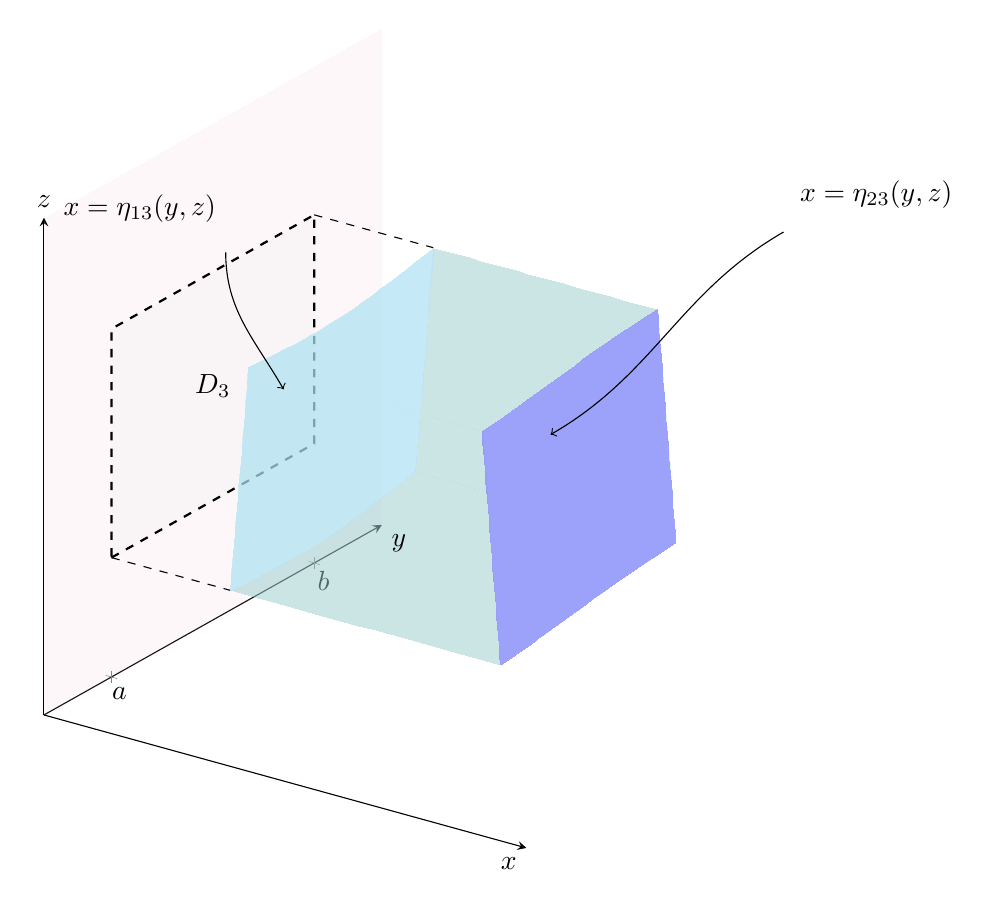
\begin{tikzpicture}
    \begin{axis}[
        view={35}{25}, 
        width=12cm, height=12cm,
        grid=none,
        axis lines=center,
        xmin=0, xmax=6, % Eje de proyección x
        ymin=0, ymax=5,
        zmin=0, zmax=5,
        xtick=\empty, ytick={1,4}, yticklabels={$a$,$b$},
        ztick=\empty,
        xlabel={$x$}, ylabel={$y$}, zlabel={$z$},
        every axis x label/.style={at={(ticklabel* cs:1)},anchor=north east},
        every axis y label/.style={at={(ticklabel* cs:1)},anchor=north west},
        every axis z label/.style={at={(ticklabel* cs:1)},anchor=south},
        clip=false
    ]

    % --- 0. Plano de fondo Lila (yz en x=0) ---
    \addplot3 [surf, domain=0:5, domain y=0:5, samples=2, opacity=0.1, colormap={lila}{color=(purple!30) color=(purple!30)}, shader=interp, draw=none] (0,x,y);

    % --- 1. Dominio D_3 en R2 (Plano yz) ---
    \addplot3 [surf, domain=1:4, domain y=1.2:3.5, samples=2, opacity=0.15, colormap={gray}{color=(gray!20) color=(gray!20)}, shader=interp, draw=none] 
        (0, x, y);
    \draw[dashed, black, thick] (0, 1, 1.2) -- (0, 4, 1.2) -- (0, 4, 3.5) -- (0, 1, 3.5) -- cycle;

    % --- 2. Paredes del volumen (Relleno completo de las 4 caras laterales) ---
    % Pared superior en z = 3.5
    \addplot3 [surf, domain=1:4, domain y=0:1, samples=20, opacity=0.3, colormap={teal}{color=(teal!40) color=(teal!40)}, shader=interp, draw=none] 
        ({ (1-y)*(1.2 + 0.2*sin(x*50) + 0.1*3.5) + y*(4.8 + 0.2*cos(x*40) - 0.1*3.5) }, x, 3.5);
    
    % Pared inferior en z = 1.2
    \addplot3 [surf, domain=1:4, domain y=0:1, samples=20, opacity=0.3, colormap={teal}{color=(teal!40) color=(teal!40)}, shader=interp, draw=none] 
        ({ (1-y)*(1.2 + 0.2*sin(x*50) + 0.1*1.2) + y*(4.8 + 0.2*cos(x*40) - 0.1*1.2) }, x, 1.2);

    % Pared lateral anterior en y = 1 (Une de z=1.2 a z=3.5)
    \addplot3 [surf, domain=1.2:3.5, domain y=0:1, samples=20, opacity=0.3, colormap={teal}{color=(teal!40) color=(teal!40)}, shader=interp, draw=none] 
        ({ (1-y)*(1.2 + 0.2*sin(1*50) + 0.1*x) + y*(4.8 + 0.2*cos(1*40) - 0.1*x) }, 1, x);

    % Pared lateral posterior en y = 4 (Une de z=1.2 a z=3.5)
    \addplot3 [surf, domain=1.2:3.5, domain y=0:1, samples=20, opacity=0.3, colormap={teal}{color=(teal!40) color=(teal!40)}, shader=interp, draw=none] 
        ({ (1-y)*(1.2 + 0.2*sin(4*50) + 0.1*x) + y*(4.8 + 0.2*cos(4*40) - 0.1*x) }, 4, x);

    % --- 3. Superficie Trasera x = eta13 ---
    \addplot3 [surf, domain=1:4, domain y=1.2:3.5, samples=25, opacity=0.6, colormap={cyan}{color=(cyan!30) color=(cyan!30)}, shader=interp, draw=none] 
        ({ 1.2 + 0.2*sin(x*50) + 0.1*y }, x, y);

    % --- 4. Superficie Delantera x = eta23 ---
    \addplot3 [surf, domain=1:4, domain y=1.2:3.5, samples=25, opacity=0.7, colormap={blue}{color=(blue!50) color=(blue!50)}, shader=interp, draw=none] 
        ({ 4.8 + 0.2*cos(x*40) - 0.1*y }, x, y);

    % --- 5. Proyecciones punteadas al plano ---
    \draw[dashed, thin] (0,1,1.2) -- ({1.2+0.2*sin(50)+0.1*1.2}, 1, 1.2);
    \draw[dashed, thin] (0,4,3.5) -- ({1.2+0.2*sin(200)+0.1*3.5}, 4, 3.5);

    % --- 6. Etiquetas y flechas optimizadas ---
    \node at (0, 2.5, 2.35) {$D_3$};
    
    % Flecha para la sábana frontal (azul)
    \node[anchor=south west] at (5.5, 4.5, 4.5) {$x = \eta_{23}(y,z)$};
    \draw[->, thin] (5.5, 4.4, 4.4) to[out=210, in=30] (4.2, 2.5, 2.8);
    
    % Flecha para la sábana trasera (cyan) - Desde arriba apuntando hacia abajo
    \node[anchor=south east] at (1.0, 1.5, 4.5) {$x = \eta_{13}(y,z)$};
    \draw[->, thin] (1.0, 1.5, 4.3) to[out=270, in=120] (1.3, 2.0, 2.8);

\end{axis}
\end{tikzpicture}
\caption{Conjunto elemental de Tipo 3.}
 
    \label{fig:Conjunto tipo 3}
\end{figure}



\newpage

\begin{example}
    Un ejemplo de un conjunto que es elemental en $\mathbb{R}^3$ es una esfera sólida (o bola) de radio $R$ centrada en el origen:
    $$W = \{(x,y,z) \in \mathbb{R}^3 \mid x^2 + y^2 + z^2 \leq R^2\}$$

    Para ver que es un conjunto elemental del primer tipo (proyección sobre el plano $xy$), identificamos primero su región de proyección $D_1$:
    $$D_1 = \{(x,y) \in \mathbb{R}^2 \mid x^2 + y^2 \leq R^2\}$$
    
    Sabemos que $D_1$ es un conjunto elemental en $\mathbb{R}^2$ (como se vio en el ejemplo de la Definición \ref{conj_elem}). Sobre esta región $D_1$, la variable $z$ queda acotada inferiormente por la semiesfera inferior y superiormente por la semiesfera superior. Es decir, existen las funciones continuas:
    $$ \eta_{11}(x,y) = -\sqrt{R^2 - x^2 - y^2} $$
    $$ \eta_{21}(x,y) = \sqrt{R^2 - x^2 - y^2} $$
    
    Tales que $\eta_{11}(x,y) \leq z \leq \eta_{21}(x,y)$ para todo $(x,y) \in D_1$. 

   Análogamente, se puede describir dicho conjunto de otras dos maneras según el plano en el que se proyecta:
\begin{enumerate}
    \item \textbf{Proyección sobre el plano $xz$:} La región elemental $D_2 \subset \mathbb{R}^2$ es el disco:
        \[
        D_2 = \{(x,z) \in \mathbb{R}^2 \mid x^2 + z^2 \leq R^2\}
        \]
        y la variable $y$ queda acotada por las funciones continuas:
        \[
        \eta_{12}(x,z) = -\sqrt{R^2 - x^2 - z^2} \quad \text{e} \quad \eta_{22}(x,z) = \sqrt{R^2 - x^2 - z^2}
        \]

    \item \textbf{Proyección sobre el plano $yz$:} La región elemental $D_3 \subset \mathbb{R}^2$ es el disco:
        \[
        D_3 = \{(y,z) \in \mathbb{R}^2 \mid y^2 + z^2 \leq R^2\}
        \]
        y la variable $x$ queda acotada por las funciones continuas:
        \[
        \eta_{13}(y,z) = -\sqrt{R^2 - y^2 - z^2} \quad \text{e} \quad \eta_{23}(y,z) = \sqrt{R^2 - y^2 - z^2}
        \]
\end{enumerate}

\begin{figure}[htbp]
    \centering
    % Llamamos al archivo con el código TikZ extraído
    
    \centering
 
    \tikzsetnextfilename{ej_esfera_elemental} 
    
    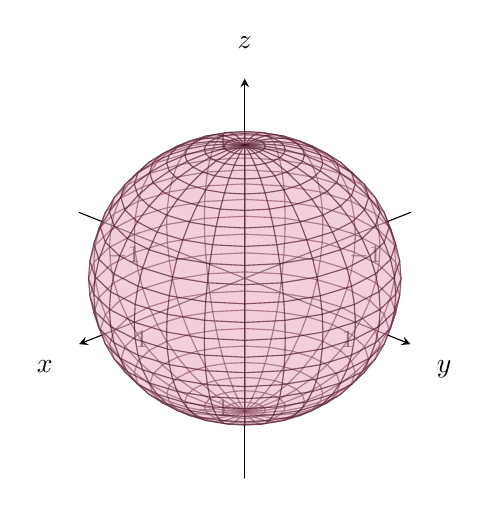
\begin{tikzpicture}[line cap=round, line join=round]
        \begin{axis}[
            view={135}{25}, % Cámara clásica
            width=10cm,
            height=10cm,
            axis lines=center,
            % Ajustamos los ejes a la esfera de radio 1
            xmin=-1.5, xmax=1.5, 
            ymin=-1.5, ymax=1.5,
            zmin=-1.5, zmax=1.5,
            xlabel={$x$},
            ylabel={$y$},
            zlabel={$z$},
            % Anclaje perfecto de letras
            every axis x label/.style={at={(ticklabel* cs:1.05)},anchor=north east},
            every axis y label/.style={at={(ticklabel* cs:1.05)},anchor=north west},
            every axis z label/.style={at={(ticklabel* cs:1.05)},anchor=south},
            ticklabel style={font=\small},
        ]

        % Esfera unitaria x^2 + y^2 + z^2 = 1 (Roja transparente)
        \addplot3[
            surf,
            opacity=0.4,
            color=purple!30,
            faceted color=purple!30!black,
            samples=25, % Reducido para no saturar la memoria
            domain=0:360,
            y domain=0:180,
            z buffer=sort
        ]
        ({cos(x)*sin(y)}, {sin(x)*sin(y)}, {cos(y)});

        \end{axis}
    \end{tikzpicture}
    \caption{Representación de la región $W$.}

 
    \label{fig:Representación de la región W}
\end{figure}
\end{example}

